\documentclass[letterpaper]{article}
\usepackage{amssymb}
\usepackage{tabularx}
\usepackage{hyperref}
\usepackage{multicol}
\usepackage{graphicx}
\usepackage[letterpaper, margin=1in]{geometry}

\usepackage{xcolor}
\hypersetup{
    colorlinks,
    linkcolor={blue!50!black},
    citecolor={blue!50!black},
    urlcolor={blue!80!black}
}

\setcounter{tocdepth}{2}

\title{18OC}
\author{Christopher Giroir}

\begin{document}

\begin{titlepage}
  \begin{center}
    \vfill
    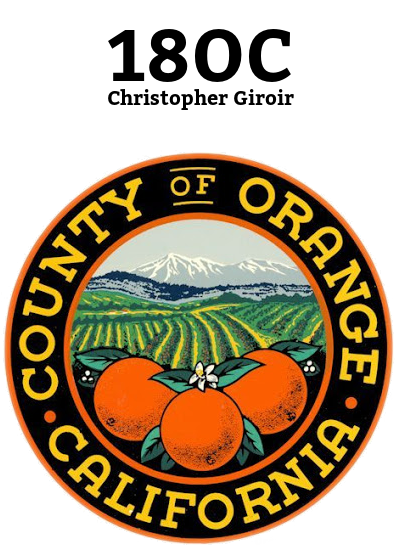
\includegraphics[width=400px]{18OC.png}
    \vfill
  \end{center}
\end{titlepage}

\newpage
\tableofcontents
\newpage

\begin{multicols}{2}
    \section{Acknowledgments}

    This game (like all 18xx) owes it's existance to Francis Tresham and his
    amazing 1829, 1830 and 1825 (as well as many others.

    This game was heavily inspire by 1817, 1871 and 1849.
\end{multicols}

\newpage

\section{Private Companies}
\begin{tabularx}{\linewidth}{l|l|l|X}
  \hline
  \textbf{Name} & \textbf{Value} & \textbf{Revenue} & \textbf{Description} \\
  \hline
  \hline
  Frozen Banana Stand & 30 & 5 & A company owning the Frozen Banana Stand gets +10 when running to Newport Beach. \\
  \hline
  Sudden Valley & 40 & 10 & When a coporation buys in Sudden Valley they may place a +10 token and a yellow tile on Mission Viejo or Lake Forest adding 10 to any company that runs to it. This tilie lay is in addition to their normal lay. \\
  \hline
  Dry the Wetlands & 70 & 15 & A corporation that owns ``Dry the Wetlands'' no longer has to pay terran cost in swamp hexes. \\
  \hline
  C.W. Swappigan's & 110 & 20 & A player owning C.W. Swappigan's may trade it for any share in a treasury or the bank poo. The bank pays current market value for a share taken from a companies treasury. \\
  \hline
  Fakeblock & 160 & 25 & A corporation buying the Fakeblock private gets a station token in Irvine. \\
  \hline
  Put up this wall & 220 & 30 & The owner of the wall private company immediately reveives the President's certificate of the CSR without further payment. The wall private company may not be sold to any corporation, and does not exchange hands if the owning player loses the Presidency of the CSR. When the CSR purchases its first train the private company is closed down. \\
  \hline
\end{tabularx}

\section{Railway Companies}
\begin{tabularx}{\linewidth}{X|l|l|l|X}
  \hline
  \textbf{Name} & \textbf{Abbrev} & \textbf{Tokens} & \textbf{Home} & \textbf{Notes} \\
  \hline
  \hline
  Disneyland Railroad & DRR & 1 & Anaheim & Always has it's home in Anaheim and is blocking regardless of it's operating status. \\
  \hline
  Santa Ana \& Newport Railway & SNR & 3 & Newport Beach & \\
  \hline
  Southern California Railway & SCR & 3 & Orange & \\
  \hline
  California Southern Railroad & CSR & 3 & San Diego & Started via the Put up this wall private. \\
  \hline
  Pacific Electric Railway Company & PE & 1 & Seal Beach & Starts operating when Seal Beach is connected to Huntington Beach. Not player owned. \\
  \hline
  Southern Pacific Railroad & SP & 5 & Los Angeles & Starts operating on the 4-train. Not player owned. \\
  \hline
  Atchison, Topeka and Santa Fe Railway & ATSF & 5 & Riverside & Starts operating on the 4-train. Not player owned. \\
  \hline
  Southern Pacific \& Santa Fe Railway & SPSF & 10 & \textit{n/a} & Possible merger from SP and ATSF. \\
  \hline
  Union Pacific Railroad & UP & 5 & Los Angeles & \\
  \hline
  BNSF Railway & BNSF & 5 & Riverside & \\
  \hline
\end{tabularx}

\newpage

\thispagestyle{empty}
\begin{multicols}{2}
    \section*{Cheat Sheet}
    \begin{tabular}{l|l|l}
      \hline
      \textbf{Players} & \textbf{Cert Limit} & \textbf{Starting Capital} \\
      \hline
      \hline
      3 & 16 & \$400 \\
      4 & 13 & \$300 \\
      \hline
    \end{tabular}
    \subsection*{Stock Round}
    \begin{itemize}
    \item Sell then Buy
    \item Never more than 50\% in the pool
    \item Can not sell shares of companies which haven't completed an operating round
    \item Companies float at 2 shares sold, partial cap.
    \end{itemize}
    \subsection*{Operating Round}

    \begin{itemize}
    \item All player owned companies must own a train
    \item Privates may be bought in from half to double face value
    \end{itemize}

    \subsubsection*{Turn Sequence}
    \begin{enumerate}
    \item Two plain or one city tile action
    \item Place a station token
    \item Run trains
    \item Pay out or withhold
    \item Acquisition \textit{(after 4-trains)}
    \item Buy trains
    \item Issue or Redeem shares \textit{(Starting 2nd OR of operation)}
    \end{enumerate}

    \subsubsection*{Stock Movement}
    \begin{tabular}{c|c}
      \hline
      \textbf{Action} & \textbf{Movement} \\
      \hline
      \hline
      Payout $= 0$ & $\leftarrow$ \\
      Payout $< SP$ & $\circlearrowright$ \\
      Payout $\geq SP$ & $\rightarrow$ \\
      Payou $\geq 2 \times SP$ & $\rightarrow\rightarrow$ \\
      \hline
      Sell Shares & $\leftarrow$ per share \\
      Issue Shares & $\leftarrow$ per share \\
      Fully Player Owned & $\rightarrow$ \\
      \hline
    \end{tabular}

    \subsection*{Companies}

    \subsubsection*{Major Companies}
    \begin{enumerate}
    \item The California Southern Railroad (CSR), Southern California Railway (SCR)
    and the Santa Ana \& Newport Railway all function as standard 10 share
    companies
    \item The CSR opens as part of the initial auction
    \item The SCR and SNR along with the DRR open in a random order
    \item When all of these companies close, they get added to the queue of companies to open
    \item Can be restarted anywhere, no longer have a reserved home (DRR excepted)
    \end{enumerate}

    \subsubsection*{Pacific Electric}
    \begin{itemize}
    \item Never player owned
    \item Operates the round after Seal Beach is connected to Huntington Beach
    \item Starts at a share price of \$100
    \item Uses currently available train from the bank pool and always pays out
    \end{itemize}
    \subsubsection*{Disneyland Railroad}
    \begin{itemize}
    \item Home token permanently on the board in Anaheim, always blocks
    \end{itemize}

    \subsection*{Acquisitions}

    \begin{itemize}
    \item Starting on the 4 train SP and ATSF get placed on the market, and
        start operating on the next OR.
    \item After running but before buying trains a company can be acquired by
        the SP or ATSF.
        \begin{enumerate}
        \item Replace tokens with tokens from acquiring company
        \item Shareholders receive current share price for each share
        \item President buys a share of acquiring company at current share price
        \item Company is added to queue of opening companies, can be started
            anywhere (no reserved home token)
        \end{enumerate}
    \end{itemize}

    \subsection*{Mergers}

    \begin{itemize}
    \item When 5 shares total are out for SP and ATSF then they attempt to merge.
    \item Each shareholder votes yes or no. Bank votes no.
    \item If it passes then all tokens are replaced with SPSF tokens and shares
        trade one for one. Stock prices average.
    \item If it fails, then SP becomes UP and shares convert to 10\%
        shares. ATSF becomes BNSF and shares convert to 10\% shares.
    \end{itemize}
\end{multicols}
\end{document}
